\documentclass[11pt,a4paper]{article}
\usepackage[T1]{fontenc}
\usepackage[margin=2.3cm]{geometry}
\usepackage{amsmath,amssymb}
\usepackage{graphicx}
\usepackage[dvipsnames]{xcolor}
\usepackage{enumitem}
\usepackage[colorlinks=true,linkcolor=blue,urlcolor=blue]{hyperref}
\setlength{\parskip}{0.6em}
\setlength{\parindent}{0pt}
\begin{document}

\begin{center}{\LARGE\bfseries openvfx}\\[0.4em]{\large Bend a character arm like a film VFX artist, in three sessions.}\\[0.2em]\small PAN IIT OSS explainer \textbullet{} secondary school to diploma / undergraduate (levels 3-5)\end{center}

\section*{Why this exists}
Every animated character is a surface of thousands of points that must follow an invisible skeleton. This explainer shows the mathematics behind that, using only rotations and matrix products, so you can build it yourself.

\section*{The end goal}
Bend a character arm for film VFX using matrix transformations and skinning. The end goal is character rigging as used in film VFX and games: a skeleton moves, and a skin that behaves like flesh follows it. The same mathematics drives robot arms and the deformation of real materials.

\section*{How the three sessions build up}
\begin{enumerate}[nosep]
\item \textbf{Session 1: One matrix moves a whole arm} (Level 1, conceptual interactive model, 60 min).
\item \textbf{Session 2: Bones rotate about joints, and joints chain} (Level 2, mathematical engineering model, 75 min).
\item \textbf{Session 3: Skin that follows the bones} (Level 3, simulation and validation, 90 min).
\end{enumerate}

\section{Session 1: One matrix moves a whole arm}

\subsection*{A. Real-world problem}
Every frame of an animated film moves thousands of points on a character. Nobody moves them one at a time: one matrix moves them all at once. When a character waves, the arm must swing round without stretching or shrinking. How do we write 'turn everything by 30 degrees' so that a computer can do it for every point?

\subsection*{B. Concept and theory}
A point is a pair of coordinates (x, y). Rotating it counter-clockwise by an angle theta about the origin gives new coordinates found from the rotation matrix R(theta). Multiplying a matrix by a point means: each new coordinate is a row of the matrix multiplied term by term with (x, y) and added. The two columns of R are unit-length and perpendicular, which is why R keeps lengths and angles; its determinant 1 says that area is kept too.

\begin{itemize}[nosep]
\item theta: rotation angle, counter-clockwise (degrees or radians)
\item (x, y): coordinates of a point (units (any length unit))
\item R: rotation matrix (no unit)
\item L: arm length (distance shoulder to hand) (units)
\end{itemize}

\begin{equation*}
R(\theta)=\begin{pmatrix}\cos\theta & -\sin\theta\\ \sin\theta & \cos\theta\end{pmatrix}
\end{equation*}

\begin{equation*}
\begin{pmatrix}x'\\ y'\end{pmatrix}=R(\theta)\begin{pmatrix}x\\ y\end{pmatrix}=\begin{pmatrix}x\cos\theta-y\sin\theta\\ x\sin\theta+y\cos\theta\end{pmatrix}
\end{equation*}

\begin{equation*}
R(\theta)^{\mathsf T}R(\theta)=I\quad\text{(columns are unit length and perpendicular, so lengths are kept)}
\end{equation*}

\begin{equation*}
\det R(\theta)=\cos^2\theta+\sin^2\theta=1\quad\text{(area is kept)}
\end{equation*}

\begin{center}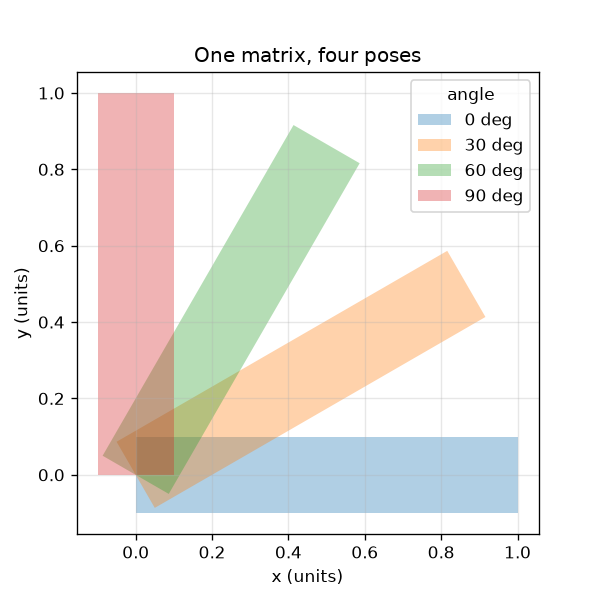
\includegraphics[width=0.85\linewidth]{figures/s01_arm_poses.png}\\\small One matrix, four poses: the arm keeps its length and thickness.\end{center}

\subsection*{E. Worked example}
Where does the hand end up after the arm (length 1, pointing along x) is turned by 30 degrees? Check that the length is still 1.
\begin{enumerate}[nosep]
\item The hand starts at (1, 0). For 30 degrees, cos = 0.866 and sin = 0.500.
\item New x = 0.866 * 1 - 0.500 * 0 = 0.866.
\item New y = 0.500 * 1 + 0.866 * 0 = 0.500.
\item Length = sqrt(0.866\textasciicircum{}2 + 0.500\textasciicircum{}2) = sqrt(0.750 + 0.250) = sqrt(1.000) = 1.
\end{enumerate}
\textbf{Answer.} The hand lands at (0.866, 0.500) and the length is still 1.

\subsection*{F. Questions}
\begin{enumerate}[nosep]
\item \textbf{Conceptual.} Why can a rotation never stretch the arm? What would a matrix that stretched the arm have to look like?
\item \textbf{Numerical.} Rotate the point (2, 0) by 90 degrees counter-clockwise. Where does it land? Check its distance from the origin.
\item \textbf{Graph and simulation interpretation.} In the graph of hand x and y against angle, at which angle do the two curves cross, and where is the hand then?
\item \textbf{Design and optimisation challenge.} An animation needs the hand to swing from pointing right to pointing straight up in exactly 3 equal steps (frames). Choose the angle for each frame and list the hand position in each.
\end{enumerate}

\section{Session 2: Bones rotate about joints, and joints chain}

\subsection*{A. Real-world problem}
When you wave, your hand travels because your forearm rides on your elbow, which rides on your shoulder. A character rig is exactly that chain of joints. Can a cartoon arm with a 30 cm upper arm and a 25 cm forearm touch a button 35 cm across and 20 cm up? And if so, with what joint angles?

\subsection*{B. Concept and theory}
Each bone turns about its own joint. To rotate about a pivot c, move the pivot to the origin, rotate, and move back. The elbow angle b is measured relative to the upper arm, so the forearm points at the sum a + b: angles add down the chain. The distance from shoulder to hand depends only on b (law of cosines).

\begin{itemize}[nosep]
\item a: shoulder angle from the x axis (degrees)
\item b: elbow angle relative to the upper arm (degrees)
\item L1: upper arm length (0.30) (m)
\item L2: forearm length (0.25) (m)
\item e, h: elbow and hand positions (x, y) (m)
\item c: pivot point of a rotation (m)
\end{itemize}

\begin{equation*}
\mathbf x'=R(\theta)(\mathbf x-\mathbf c)+\mathbf c
\end{equation*}

\begin{equation*}
\mathbf e=L_1(\cos a,\ \sin a),\qquad \mathbf h=\mathbf e+L_2\big(\cos(a+b),\ \sin(a+b)\big)
\end{equation*}

\begin{equation*}
|\mathbf h|^2=L_1^2+L_2^2+2L_1L_2\cos b
\end{equation*}

\begin{center}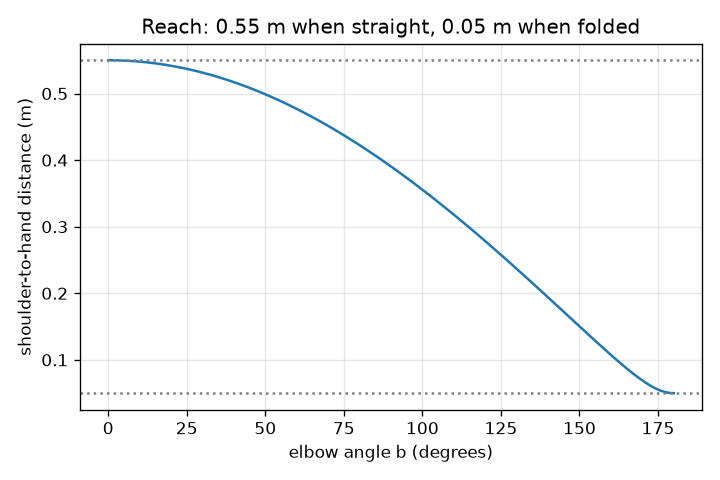
\includegraphics[width=0.85\linewidth]{figures/s02_reach_vs_elbow.png}\\\small Reach against elbow angle: 0.55 m when straight, 0.05 m when folded.\end{center}

\subsection*{E. Worked example}
With L1 = 0.30 m, L2 = 0.25 m, a = 40 degrees and b = 50 degrees, find the elbow, the hand and the shoulder-to-hand distance.
\begin{enumerate}[nosep]
\item Elbow = 0.30 * (cos 40, sin 40) = 0.30 * (0.766, 0.643) = (0.230, 0.193) m.
\item The forearm points at a + b = 90 degrees, so its offset is 0.25 * (cos 90, sin 90) = (0, 0.25) m.
\item Hand = elbow + offset = (0.230, 0.443) m.
\item Check with the reach formula: \textbar{}h\textbar{}\textasciicircum{}2 = 0.09 + 0.0625 + 2*0.30*0.25*cos 50 = 0.1525 + 0.0964 = 0.2489, so \textbar{}h\textbar{} = 0.499 m.
\item Check with the coordinates: sqrt(0.230\textasciicircum{}2 + 0.443\textasciicircum{}2) = 0.499 m. The two methods agree.
\end{enumerate}
\textbf{Answer.} Elbow (0.230, 0.193) m, hand (0.230, 0.443) m, distance 0.499 m.

\subsection*{F. Questions}
\begin{enumerate}[nosep]
\item \textbf{Conceptual.} Why does the forearm point at angle a + b rather than just b?
\item \textbf{Numerical.} For L1 = 0.30 m, L2 = 0.25 m, a = 90 degrees and b = -90 degrees, find the hand position and its distance from the shoulder.
\item \textbf{Graph and simulation interpretation.} From the reach graph, what are the largest and smallest shoulder-to-hand distances, and at which elbow angles?
\item \textbf{Design and optimisation challenge.} Design: find joint angles that put the hand on (0.35, 0.20) m. How many solutions are there? Is (1.0, 0.0) m reachable?
\end{enumerate}

\section{Session 3: Skin that follows the bones}

\subsection*{A. Real-world problem}
A skeleton has no surface. The skin is a cloud of points and each point must decide which bone to follow. If every point follows exactly one bone, the elbow cracks open like a robot's. If points follow a weighted blend of two bones, the skin looks like flesh, but the elbow gets thinner when it bends. Game engines and film studios use this method (linear blend skinning) and fight this thinning every day. Can you measure it, predict it, and keep it within limits?

\subsection*{B. Concept and theory}
Bone 1 stays put. Bone 2 turns by the bend angle b about the elbow. Each skin point has a weight w between 0 and 1 telling how much it follows bone 2. The new position is the weighted average of where bone 1 and bone 2 would put it. Smooth weights (a smoothstep ramp over a blend zone of half-width z) remove cracks. At the elbow w = 1/2, and averaging a point on the top edge with a point on the bottom edge shrinks their distance to cos(b/2) of the rest width.

\begin{itemize}[nosep]
\item b: elbow bend angle (degrees)
\item w: weight: how much a point follows bone 2 (no unit)
\item z: half-width of the blend zone (units (arm length 2))
\item h: half thickness of the arm (0.15) (units)
\item gap: largest distance between neighbouring skin points (units)
\item ratio: elbow width divided by rest width (0.30) (no unit)
\end{itemize}

\begin{equation*}
\mathbf v'=(1-w)\,\mathbf v+w\,\big(R(b)(\mathbf v-\mathbf c)+\mathbf c\big)
\end{equation*}

\begin{equation*}
w(x)=3t^2-2t^3,\qquad t=\mathrm{clip}\!\left(\frac{x-(1-z)}{2z},\,0,\,1\right)
\end{equation*}

\begin{equation*}
\text{elbow width ratio}=\cos\!\left(\frac{b}{2}\right)
\end{equation*}

\begin{center}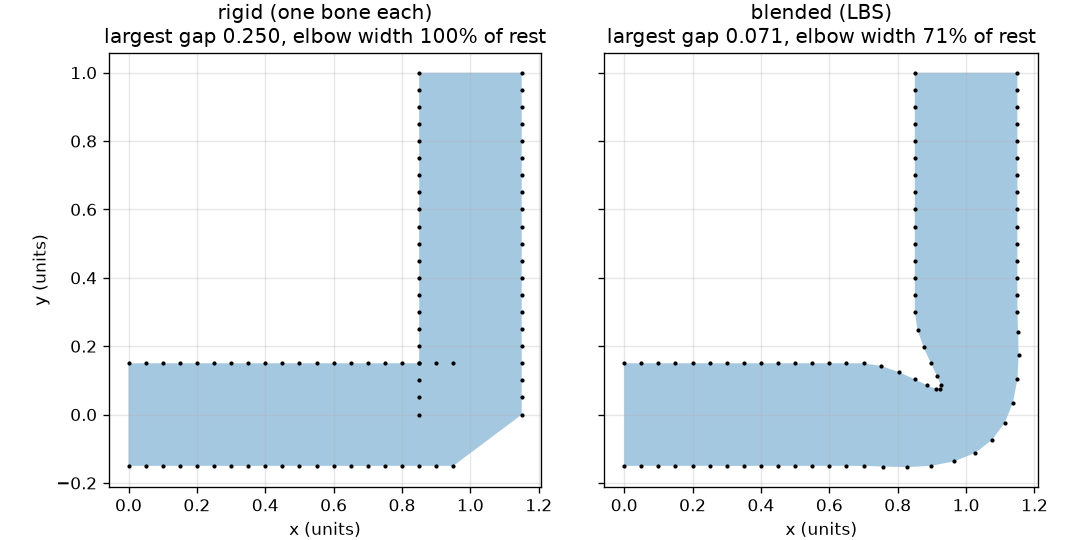
\includegraphics[width=0.85\linewidth]{figures/s03_skinning_90deg.png}\\\small A 90 degree bend: one bone per point (cracks) versus blended weights (thinner elbow).\end{center}

\subsection*{E. Worked example}
For a bend of 90 degrees and half thickness h = 0.15, find the blended elbow width and compare it with the hand-calculation cos(b/2).
\begin{enumerate}[nosep]
\item At the elbow x = 1 the weight is w = 1/2. Bone 1 keeps the top point at (1, 0.15); bone 2 turns it about the elbow to (0.85, 0).
\item Blended top point = average = (0.925, 0.075). In the same way the bottom point blends (1, -0.15) and (1.15, 0) into (1.075, -0.075).
\item Width = distance between them = sqrt(0.15\textasciicircum{}2 + 0.15\textasciicircum{}2) = 0.212.
\item Rest width = 2h = 0.30, so the ratio is 0.212 / 0.30 = 0.707.
\item Hand calculation: cos(90 / 2) = cos 45 = 0.707. They agree.
\end{enumerate}
\textbf{Answer.} The elbow keeps 70.7 percent of its width; the one-bone skin keeps 100 percent but cracks (largest gap 0.25 against a rest gap of 0.05).

\subsection*{F. Questions}
\begin{enumerate}[nosep]
\item \textbf{Conceptual.} Why does averaging the positions from two bones make the elbow thinner, while following a single bone does not?
\item \textbf{Numerical.} Use the hand calculation to find the elbow width ratio at a bend of 120 degrees. What width is that for an arm 0.30 thick?
\item \textbf{Graph and simulation interpretation.} On the width graph, at about which bend does the blue curve cross the red 80 percent line? What does that tell an animator?
\item \textbf{Design and optimisation challenge.} Design: choose a blend zone and the largest whole-degree bend so that the elbow keeps at least 80 percent width and the largest gap stays below 0.08. Justify your choice.
\end{enumerate}

\section{Real-world mini-project}
\textbf{Rig and animate a waving cartoon arm.} A studio hands you a cartoon arm and a four-frame wave: elbow bends of 0, 40, 70 and 40 degrees. The arm must not crack open and must not look thin. Use \texttt{lbs\_pose} from Session 3 and find the smallest blend zone (in steps of 0.05) for which all four frames pass.

\section{The path ahead}
\begin{enumerate}[nosep]
\item \textbf{Session 4: Helper bones at the elbow.} A three-bone arm (upper arm, helper, forearm) skinned with weights.
\item \textbf{Session 5: Paint the weights.} A small weight editor with a sliders-per-region interface that reports gap and width.
\item \textbf{Session 6: Blend rotations, not matrices (2D).} A second skinning function with constant width along the arm.
\item \textbf{Session 7: Go 3D: twist and quaternions.} The same arm in 3D with a twisting forearm.
\item \textbf{Session 8: Animate a wave cycle.} A looping animation exported as a GIF.
\end{enumerate}

\section{Answers and hints}

\subsection*{Session 1}
\begin{enumerate}[nosep]
\item \textbf{Conceptual.} Hint: Look at the length of each column of R, and ask what the determinant does and does not tell you. Solution: Each column of R is a vector of length 1 and the two columns are perpendicular (R\textasciicircum{}T R = I), so R keeps lengths and angles. The determinant cos\textasciicircum{}2 + sin\textasciicircum{}2 = 1 only tells us that area is kept: a shear such as [[1, 1], [0, 1]] also has determinant 1 but stretches things (it sends (1, 1) to (2, 1)). A matrix that stretches the arm, such as [[2, 0], [0, 1]] which doubles x, has a column longer than 1.
\item \textbf{Numerical.} Hint: For 90 degrees cos = 0 and sin = 1. Apply new x = x cos - y sin and new y = x sin + y cos. Solution: new x = 2*0 - 0*1 = 0 and new y = 2*1 + 0*0 = 2, so the point lands at (0, 2). Distance = sqrt(0\textasciicircum{}2 + 2\textasciicircum{}2) = 2, the same as before. Units: same unit as the input.
\item \textbf{Graph and simulation interpretation.} Hint: They cross where cos = sin. Solution: They cross at 45 degrees (and again at 225 degrees). At 45 degrees x = y = 0.707, so the hand is at (0.707, 0.707). Reading the graph, both curves have the value 0.707 there.
\item \textbf{Design and optimisation challenge.} Hint: The total turn is 90 degrees; divide it into three equal steps and use R for each cumulative angle. Solution: Each step is 30 degrees, so the frames are at 30, 60 and 90 degrees. Hand positions: (0.866, 0.500), (0.500, 0.866) and (0.000, 1.000). Assumption: constant speed. A real animator would also ease in and out.
\end{enumerate}

\subsection*{Session 2}
\begin{enumerate}[nosep]
\item \textbf{Conceptual.} Hint: Where is the elbow angle b measured from? Solution: b is measured relative to the upper arm, not relative to the x axis. The upper arm already points at a, so the forearm points at a plus whatever extra turn the elbow adds. Angles accumulate down the chain.
\item \textbf{Numerical.} Hint: The forearm points at a + b = 0 degrees. Solution: Elbow = 0.30 * (0, 1) = (0, 0.30) m. Forearm offset = 0.25 * (1, 0) = (0.25, 0). Hand = (0.25, 0.30) m. Distance = sqrt(0.0625 + 0.09) = 0.391 m. Check: reach formula gives sqrt(0.1525 + 0.15 cos(-90)) = sqrt(0.1525) = 0.391 m.
\item \textbf{Graph and simulation interpretation.} Hint: Read the highest and lowest points of the curve and the matching x values. Solution: The largest is 0.55 m = L1 + L2 at b = 0 degrees (straight arm). The smallest is 0.05 m = \textbar{}L1 - L2\textbar{} at b = 180 degrees (forearm folded back). Both are the ends of the curve, where cos b = 1 and -1.
\item \textbf{Design and optimisation challenge.} Hint: First find b from \textbar{}h\textbar{}\textasciicircum{}2 = 0.35\textasciicircum{}2 + 0.20\textasciicircum{}2 using the reach formula, then find a. Solution: \textbar{}h\textbar{}\textasciicircum{}2 = 0.1625, so cos b = (0.1625 - 0.1525) / 0.15 = 0.0667 and b = +86.2 or -86.2 degrees. For each b, a = atan2(0.20, 0.35) - atan2(0.25 sin b, 0.30 + 0.25 cos b): a = -8.5 degrees for b = +86.2 (elbow down) and a = 68.0 degrees for b = -86.2 (elbow up). Two solutions. (1.0, 0.0) is 1 m away but the longest reach is 0.55 m, so it is unreachable.
\end{enumerate}

\subsection*{Session 3}
\begin{enumerate}[nosep]
\item \textbf{Conceptual.} Hint: Picture the top and bottom points ending up near each other after the two bones turn them in different directions. Solution: Following one bone moves a top point and its matching bottom point by the same rigid motion, so their distance does not change. Averaging two different motions pulls a top point and a bottom point towards the middle: the average of two rotated points is closer to the centre than either, so the distance between them shrinks. Averaging matrices is not a rotation any more.
\item \textbf{Numerical.} Hint: ratio = cos(b/2). Solution: ratio = cos(60 degrees) = 0.5. Width = 0.5 * 0.30 = 0.15 (units). The elbow has lost half its width, much worse than at 90 degrees.
\item \textbf{Graph and simulation interpretation.} Hint: Solve cos(b/2) = 0.8. Solution: b/2 = arccos(0.8) = 36.9 degrees, so b = 73.7 degrees. Below about 74 degrees the elbow keeps at least 80 percent of its width; above it, the skin looks visibly pinched. An animator must limit the bend or add helper bones.
\item \textbf{Design and optimisation challenge.} Hint: Use lbs\_pose(bend, zone) and print the gap and width ratio for a few zones and bends. Solution: Width needs cos(b/2) \textgreater{}= 0.8, so b \textless{}= 73.7 degrees: the largest whole-degree bend is 73. At 73 degrees with zone 0.2 the largest gap is 0.075 (below 0.08), so zone 0.2 works; zone 0.15 gives 0.083 at 70 degrees and fails. A safer choice with margin is zone 0.3 and bends up to 70 degrees: width 0.82, gap 0.067. Trade-off: a wider zone reduces the gap but blurs where the elbow is.
\end{enumerate}

\section{How to join}
Read \texttt{CONTRIBUTING.md} in the repository, then pick an issue labelled \texttt{good first issue}. Repository: \url{https://github.com/KrunalPanchal1995/openvfx}

\end{document}
